%definira klasu dokumenta 
\documentclass[12pt]{report} 

%prostor izmedu naredbi \documentclass i \begin{document} se zove uvod. U njemu se nalaze naredbe koje se odnose na cijeli dokument

%osnovni LaTex ne može riješiti sve probleme, pa se koriste različiti paketi koji olakšavaju izradu željenog dokumenta
\usepackage[croatian]{babel} 
\usepackage{amssymb}
\usepackage{amsmath}
\usepackage{txfonts}
\usepackage{mathdots}
\usepackage{titlesec}
\usepackage{array}
\usepackage{lastpage}
\usepackage{etoolbox}
\usepackage{tabularray}
\usepackage{color, colortbl}
\usepackage{adjustbox}
\usepackage{geometry}
\usepackage[classicReIm]{kpfonts}
\usepackage{hyperref}
\usepackage{fancyhdr}

\usepackage{float}
\usepackage{setspace}
\restylefloat{table}


\patchcmd{\chapter}{\thispagestyle{plain}}{\thispagestyle{fancy}}{}{} %redefiniranje stila stranice u paketu fancyhdr

%oblik naslova poglavlja
\titleformat{\chapter}{\normalfont\huge\bfseries}{\thechapter.}{20pt}{\Huge}
\titlespacing{\chapter}{0pt}{0pt}{40pt}


\linespread{1.3} %razmak između redaka

\geometry{a4paper, left=1in, top=1in,}  %oblik stranice

\hypersetup{ colorlinks, citecolor=black, filecolor=black, linkcolor=black,	urlcolor=black }   %izgled poveznice


%prored smanjen između redaka u nabrajanjima i popisima
\newenvironment{packed_enum}{
	\begin{enumerate}
		\setlength{\itemsep}{0pt}
		\setlength{\parskip}{0pt}
		\setlength{\parsep}{0pt}
	}{\end{enumerate}}

\newenvironment{packed_item}{
	\begin{itemize}
		\setlength{\itemsep}{0pt}
		\setlength{\parskip}{0pt}
		\setlength{\parsep}{0pt}
	}{\end{itemize}}




%boja za privatni i udaljeni kljuc u tablicama
\definecolor{LightBlue}{rgb}{0.9,0.9,1}
\definecolor{LightGreen}{rgb}{0.9,1,0.9}

%Promjena teksta za dugačke tablice
\DefTblrTemplate{contfoot-text}{normal}{Nastavljeno na idućoj stranici}
\SetTblrTemplate{contfoot-text}{normal}
\DefTblrTemplate{conthead-text}{normal}{(Nastavljeno)}
\SetTblrTemplate{conthead-text}{normal}
\DefTblrTemplate{middlehead,lasthead}{normal}{Nastavljeno od prethodne stranice}
\SetTblrTemplate{middlehead,lasthead}{normal}

%podesavanje zaglavlja i podnožja

\pagestyle{fancy}
\lhead{Programsko inženjerstvo}
\rhead{Dog Friendly}
\lfoot{Monty Python}
\cfoot{stranica \thepage/\pageref{LastPage}}
\rfoot{\today}
\renewcommand{\headrulewidth}{0.2pt}
\renewcommand{\footrulewidth}{0.2pt}


\begin{document} 
	
	
	
	\begin{titlepage}
		\begin{center}
			\vspace*{\stretch{1.0}} %u kombinaciji s ostalim \vspace naredbama definira razmak između redaka teksta
			\LARGE Programsko inženjerstvo\\
			\large Ak. god. 2022./2023.\\
			
			\vspace*{\stretch{3.0}}
			
			\huge Dog Friendly\\
			\Large Dokumentacija, Rev. 1\\
			
			\vspace*{\stretch{12.0}}
			\normalsize
			Grupa: \textit{MontyPython}\\
			Voditelj: \textit{Fran Markulin}\\
			
			
			\vspace*{\stretch{1.0}}
			Datum predaje: \textit{18.11.2022.}\\
	
			\vspace*{\stretch{4.0}}
			
			Nastavnik: \textit{Laura Majer}\\
		
		\end{center}

	
	\end{titlepage}

	
	\tableofcontents


	\chapter{Dnevnik promjena dokumentacije}
		
		%\textbf{\textit{Kontinuirano osvježavanje}}\\
				
		
		\begin{longtblr}[
				label=none
			]{
				width = \textwidth, 
				colspec={|X[2]|X[13]|X[3]|X[3]|}, 
				rowhead = 1
			}
			\hline
			\textbf{Rev.}	& \textbf{Opis promjene/dodatka} & \textbf{Autori} & \textbf{Datum}\\[3pt] \hline
			0.1 & Napravljen predložak.	& Jura Starčević & 5.11.2022. 		\\[3pt] \hline 
			0.2	& Dodan opis & Jura Starčević & 6.11.2022. 	\\[3pt] \hline 
			0.3 & Dodano i djelomično uređeno poglavlje 3.1 & Marko Štrk & 8.11.2022. \\[3pt] \hline 
			0.4 & Početak dodavanja informacija o bazi & Jura Starčević & 15.11.2022. \\[3pt] \hline 
			0.5 & Dodan djelomičan dijagram obrazaca uporabe & Karla Udiljak & 15.11.2022. \\[3pt] \hline 
			0.6 & Dodani i razrađeni Use Caseovi & Marko Štrk & 16.11.2022. \\[3pt] \hline 
			0.7 & Dodavanje arhitekture i opisa baze podataka & Fran Markulin & 16.11.2022. \\[3pt] \hline 
			0.8 & Uređivanje opisa i arhitekture & Jura Starčević & 16.11.2022. \\[3pt] \hline 
			0.9 & Dodavanje potpunog dijagrama obrazaca uporabe, sekvencijskih dijagrama te njihovih opisa & Karla Udiljak & 16.11.2022. \\[3pt] \hline 
			0.10 & Dodani Ostali zahtjevi i UML dijagram & Marko Štrk & 17.11.2022. \\[3pt] \hline 
			\textbf{1.0} & Finalna verzija za prvi ciklus & Jura Starčević & 18.11.2022. \\[3pt] \hline 
           1.1 & Dodano poglavlje 6. - Zaključak i budući rad & Marko Štrk & 21.12.2022. \\[3pt] \hline 
           1.2 & Dodano i uređeno poglavlje 5.2.2 i  5.4 Upute za puštanje u pogon & Marko Štrk & 8.1.2023. \\[3pt] \hline 
		   1.3 & Uređen opis baze  & Jura Starčević & 12.1.2023. \\[3pt] \hline
         1.4 & Dodani opisi dijagrama  & Marko Štrk & 13.1.2023. \\[3pt] \hline
			
		\end{longtblr}
	
	
		%\textit{Moraju postojati glavne revizije dokumenata 1.0 i 2.0 na kraju prvog i drugog ciklusa. Između tih revizija mogu postojati manje revizije već prema tome kako se dokument bude nadopunjavao. Očekuje se da nakon svake značajnije promjene (dodatka, izmjene, uklanjanja dijelova teksta i popratnih grafičkih sadržaja) dokumenta se to zabilježi kao revizija. Npr., revizije unutar prvog ciklusa će imati oznake 0.1, 0.2, …, 0.9, 0.10, 0.11.. sve do konačne revizije prvog ciklusa 1.0. U drugom ciklusu se nastavlja s revizijama 1.1, 1.2, itd.}
	\chapter{Opis projektnog zadatka}
		
		\textbf{\textit{dio 1. revizije}}\\
		
		\textit{Na osnovi projektnog zadatka detaljno opisati korisničke zahtjeve. Što jasnije opisati cilj projektnog zadatka, razraditi problematiku zadatka, dodati nove aspekte problema i potencijalnih rješenja. Očekuje se minimalno 3, a poželjno 4-5 stranica opisa.	Teme koje treba dodatno razraditi u ovom poglavlju su:}
		\begin{packed_item}
			\item \textit{potencijalna korist ovog projekta}
			\item \textit{postojeća slična rješenja (istražiti i ukratko opisati razlike u odnosu na zadani zadatak). Dodajte slike koja predočavaju slična rješenja.}
			\item \textit{skup korisnika koji bi mogao biti zainteresiran za ostvareno rješenje.}
			\item \textit{mogućnost prilagodbe rješenja }
			\item \textit{opseg projektnog zadatka}
			\item \textit{moguće nadogradnje projektnog zadatka}
		\end{packed_item}
		
		\textit{Za pomoć pogledati reference navedene u poglavlju „Popis literature“, a po potrebi konzultirati sadržaj na internetu koji nudi dobre smjernice u tom pogledu.}
		\eject
		
		\section{Primjeri u \LaTeX u}
		
		\textit{Ovo potpoglavlje izbrisati.}\\

		U nastavku se nalaze različiti primjeri kako koristiti osnovne funkcionalnosti \LaTeX a koje su potrebne za izradu dokumentacije. Za dodatnu pomoć obratiti se asistentu na projektu ili potražiti upute na sljedećim web sjedištima:
		\begin{itemize}
			\item Upute za izradu diplomskog rada u \LaTeX u - \url{https://www.fer.unizg.hr/_download/repository/LaTeX-upute.pdf}
			\item \LaTeX\ projekt - \url{https://www.latex-project.org/help/}
			\item StackExchange za Tex - \url{https://tex.stackexchange.com/}\\
		
		\end{itemize} 	


		
		\noindent \underbar{podcrtani tekst}, \textbf{podebljani tekst}, 	\textit{nagnuti tekst}\\
		\noindent \normalsize primjer \large primjer \Large primjer \LARGE {primjer} \huge {primjer} \Huge primjer \normalsize
				
		\begin{packed_item}
			
			\item  primjer
			\item  primjer
			\item  primjer
			\item[] \begin{packed_enum}
				\item primjer
				\item[] \begin{packed_enum}
					\item[1.a] primjer
					\item[b] primjer
				\end{packed_enum}
				\item primjer
			\end{packed_enum}
			
		\end{packed_item}
		
		\noindent primjer url-a: \url{https://www.fer.unizg.hr/predmet/proinz/projekt}
		
		\noindent posebni znakovi: \# \$ \% \& \{ \} \_ 
		$|$ $<$ $>$ 
		\^{} 
		\~{} 
		$\backslash$ 
		
		
		\begin{longtblr}[
			label=none,
			entry=none
			]{
				width = \textwidth,
				colspec={|X[8,l]|X[8, l]|X[16, l]|}, 
				rowhead = 1,
			} %definicija širine tablice, širine stupaca, poravnanje i broja redaka naslova tablice
			\hline \multicolumn{3}{|c|}{\textbf{naslov unutar tablice}}	 \\ \hline[3pt]
			\SetCell{LightGreen}IDKorisnik & INT	&  	Lorem ipsum dolor sit amet, consectetur adipiscing elit, sed do eiusmod  	\\ \hline
			korisnickoIme	& VARCHAR &   	\\ \hline 
			email & VARCHAR &   \\ \hline 
			ime & VARCHAR	&  		\\ \hline 
			\SetCell{LightBlue} primjer	& VARCHAR &   	\\ \hline 
		\end{longtblr}
		

		\begin{longtblr}[
				caption = {Naslov s referencom izvan tablice},
				entry = {Short Caption},
			]{
				width = \textwidth, 
				colspec = {|X[8,l]|X[8,l]|X[16,l]|}, 
				rowhead = 1,
			}
			\hline
			\SetCell{LightGreen}IDKorisnik & INT	&  	Lorem ipsum dolor sit amet, consectetur adipiscing elit, sed do eiusmod  	\\ \hline
			korisnickoIme	& VARCHAR &   	\\ \hline 
			email & VARCHAR &   \\ \hline 
			ime & VARCHAR	&  		\\ \hline 
			\SetCell{LightBlue} primjer	& VARCHAR &   	\\ \hline 
		\end{longtblr}
	


		
		
		%unos slike
		\begin{figure}[H]
			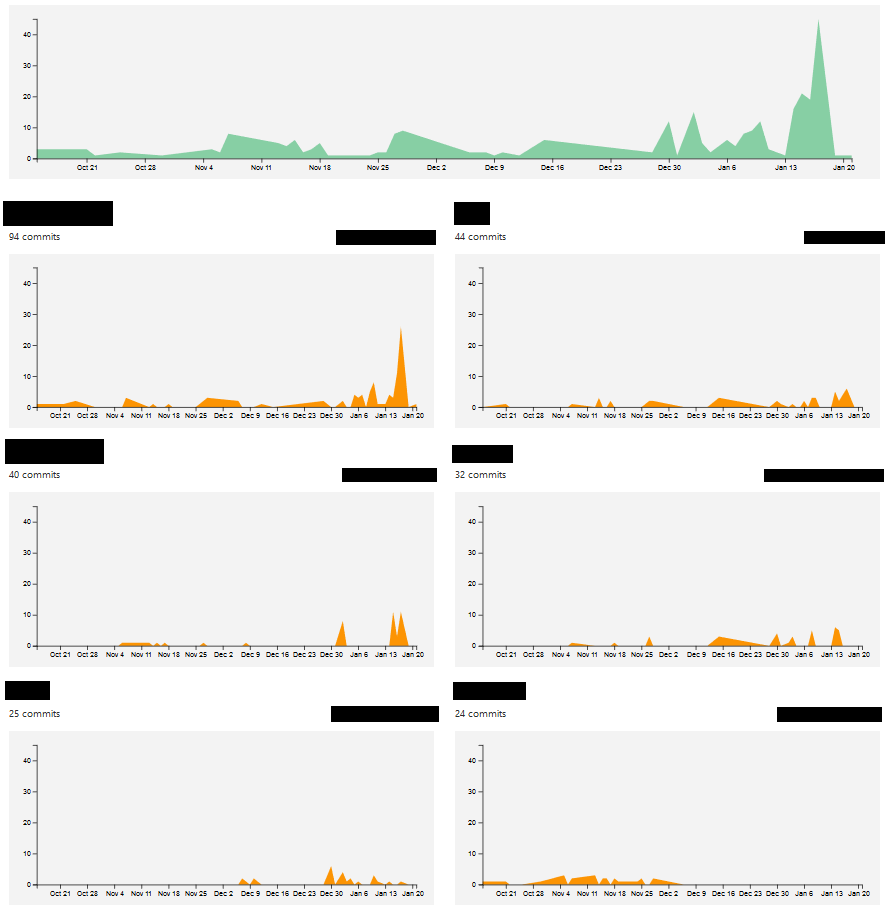
\includegraphics[scale=0.4]{slike/aktivnost.PNG} %veličina slike u odnosu na originalnu datoteku i pozicija slike
			\centering
			\caption{Primjer slike s potpisom}
			\label{fig:promjene}
		\end{figure}
		
		\begin{figure}[H]
			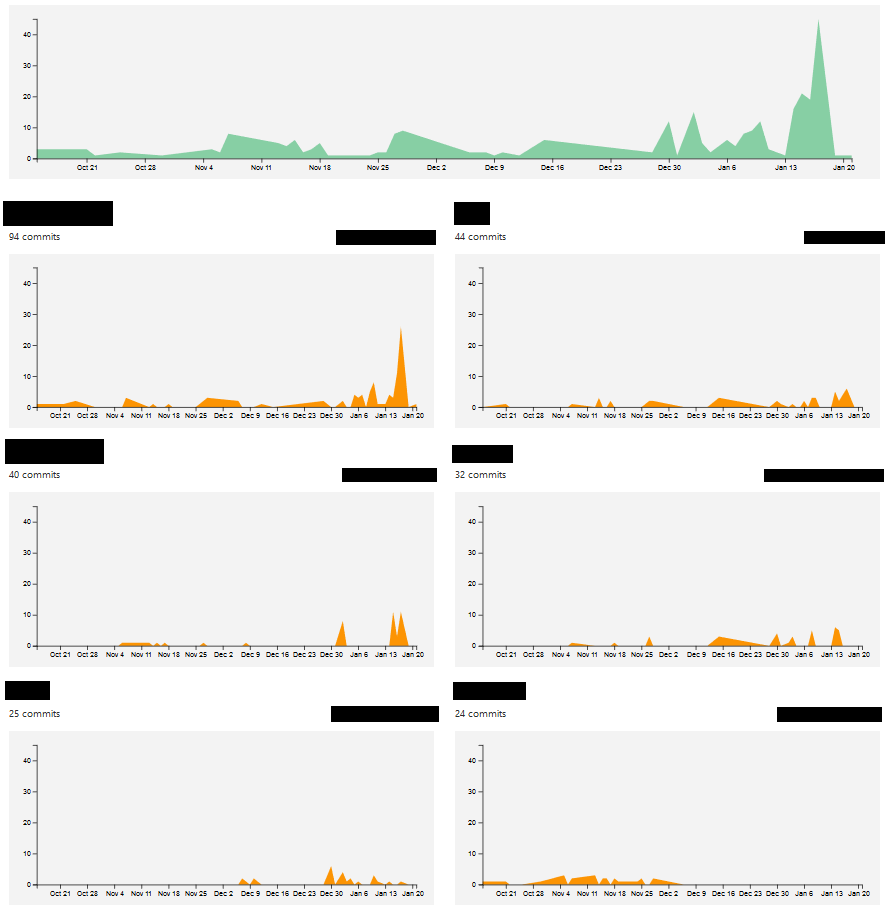
\includegraphics[width=\textwidth]{slike/aktivnost.PNG} %veličina u odnosu na širinu linije
			\caption{Primjer slike s potpisom 2}
			\label{fig:promjene2} %label mora biti drugaciji za svaku sliku
		\end{figure}
		
		Referenciranje slike \ref{fig:promjene2} u tekstu.
		
		\eject
		
	
	\chapter{Specifikacija programske potpore}
		
	\section{Funkcionalni zahtjevi}
			
			\textbf{\textit{dio 1. revizije}}\\
			
			\textit{Navesti \textbf{dionike} koji imaju \textbf{interes u ovom sustavu} ili  \textbf{su nositelji odgovornosti}. To su prije svega korisnici, ali i administratori sustava, naručitelji, razvojni tim.}\\
				
			\textit{Navesti \textbf{aktore} koji izravno \textbf{koriste} ili \textbf{komuniciraju sa sustavom}. Oni mogu imati inicijatorsku ulogu, tj. započinju određene procese u sustavu ili samo sudioničku ulogu, tj. obavljaju određeni posao. Za svakog aktora navesti funkcionalne zahtjeve koji se na njega odnose.}\\
			
			
			\noindent \textbf{Dionici:}
			
			\begin{packed_enum}
				
				\item Vlasnik (naručitelj)
				\item Vlasnik psa
				\item Vlasnik obrta
				\item Administrator
				\item Razvojni tim
				
			\end{packed_enum}
			
			\noindent \textbf{Aktori i njihovi funkcionalni zahtjevi:}
			
			
			\begin{packed_enum}
				\item  \underbar{Neregistriran/neprijavljeni korisnik može:}
				
				\begin{packed_enum}
					
					\item pregledati lokacije na karti
					\item odabrati lokaciju i dobiti prikaz opcih informacija (ime lokacije, adresa, telefon, OIB, kratak opis, djelatnost)
					\item se registrirati u sustav, stvoriti novi korisnicki račun za koji su mu potrebni korisničko ime, lozinka, ime, prezime, broj mobitela, e-mail adresa
					
					
				\end{packed_enum}
			
				\item  \underbar{Klijent(inicijator) može:}
				
				\begin{packed_enum}
					
					\item pregledavati i mijenjati osobne podatke
					\item izbrisati svoj korisnični račun
					\item pisati recentije i dati ocjene
					\item pregledati recenzije
					
				\end{packed_enum}
				
				\item  \underbar{Administrator može:}
				
				\begin{packed_enum}
					
					\item vidjeti popis svih registriranih korisnika i njihovih osobnih podataka
					\item korisnike brisati i mijenjati im razinu pristupa aplikaciji (klijent, vlasnik psa, vlasnik obrta)
					\item brisati recenzije koje su u suprotnosti s pravilima koristenja aplikacije
					\item dodati ili obrisati lokaciju
					
				\end{packed_enum}
				
				\item  \underbar{Baza podataka(sudionik):}
				
				\begin{packed_enum}
					
					\item pohranjuje sve podatke o korisnicima i njihovim ovlastima
					\item pohranjuje sve podatke o lokacijama

					
				\end{packed_enum}
				
			\end{packed_enum}
			
			\eject 
			
			
				
			\subsection{Obrasci uporabe}
				
				\textbf{\textit{dio 1. revizije}}
				
				\subsubsection{Opis obrazaca uporabe}
					\textit{Funkcionalne zahtjeve razraditi u obliku obrazaca uporabe. Svaki obrazac je potrebno razraditi prema donjem predlošku. Ukoliko u nekom koraku može doći do odstupanja, potrebno je to odstupanje opisati i po mogućnosti ponuditi rješenje kojim bi se tijek obrasca vratio na osnovni tijek.}\\
					

					\noindent \underbar{\textbf{UC1 - Pregled restorana}}
					\begin{packed_item}
	
						\item \textbf{Glavni sudionik: }Korisnik, klijent
						\item  \textbf{Cilj:} Pregledati lokacije i osnovne informacije
						\item  \textbf{Sudionici:} Baza podataka
						\item  \textbf{Preduvjet:} -
						\item  \textbf{Opis osnovnog tijeka:}
						
						\item[] \begin{packed_enum}
	
							\item Karta je prikazana prilikom učitavanja aplikacije
							\item Korisnik na karti odabire lokaciju
							\item Prikazuju se informacije o lokaciji i ponudi

						\end{packed_enum}
						
					\end{packed_item}
					
					\noindent \underbar{\textbf{UC2 - Registracija}}
					\begin{packed_item}
	
						\item \textbf{Glavni sudionik: }Korisnik
						\item  \textbf{Cilj:} Stvoriti korisnički račun za pristup sustavu
						\item  \textbf{Sudionici:} Baza podataka
						\item  \textbf{Preduvjet:} -
						\item  \textbf{Opis osnovnog tijeka:}
						
						\item[] \begin{packed_enum}
	
							\item Korisnik odabire opciju za registraciju
							\item Korisnik unosi potrebne korisničke podatke
							\item Korisnik prima e-mail za potvrdu registracije
							\item Korisnik potvrđuje registraciju
							\item Korisnik prima obavijest o uspješnoj registraciji

						\end{packed_enum}
						
						\item  \textbf{Opis mogućih odstupanja:}
						
						\item[] \begin{packed_item}
	
							\item[2.a] Odabir već zauzetog korisničkog imena i/ili e-maila, unos korisničkog podatka u nedozvoljenom formatu ili pružanje neispravnog e-maila
							\item[] \begin{packed_enum}
								
								\item Sustav obajveštava korisnika o neuspjelom upisu i vraća ga na stranicu za registraciju
								\item Korisnik mijenja podatke te završava unos ili odustaje od registracije
								
							\end{packed_enum}
							
						\end{packed_item}
					\end{packed_item}
					
					\noindent \underbar{\textbf{UC3 - Prijava u sustav}}
					\begin{packed_item}
	
						\item \textbf{Glavni sudionik: } Klijent
						\item  \textbf{Cilj:} Dobiti pristup korisničkom sučelju
						\item  \textbf{Sudionici:} Baza podataka
						\item  \textbf{Preduvjet:} Registracija
						\item  \textbf{Opis osnovnog tijeka:}
						
						\item[] \begin{packed_enum}
	
							\item Unos korisničkog imena i lozinke
							\item Potvrda ispravnosti unesenih podataka
							\item Pristup korisničkim funkcijama

						\end{packed_enum}
						
						\item  \textbf{Opis mogućih odstupanja:}
						
						\item[] \begin{packed_item}
	
							\item[2.a] Neispravno korisničko ime/lozinka
							\item[] \begin{packed_enum}
								
								\item Sustav obavještava korisnika o neuspjelom upisu i vraća ga na stranicu za registraciju
								
							\end{packed_enum}

						\end{packed_item}
					\end{packed_item}
					
					\noindent \underbar{\textbf{UC4 - Pregled osobnih podataka}}
					\begin{packed_item}
	
						\item \textbf{Glavni sudionik: } Klijent
						\item  \textbf{Cilj:} Pregledati osobne podatke
						\item  \textbf{Sudionici:} Baza podataka
						\item  \textbf{Preduvjet:} Klijent je prijavljen
						\item  \textbf{Opis osnovnog tijeka:}
						
						\item[] \begin{packed_enum}
	
							\item Korisnik odabire opciju "Osobni podatci"
							\item Aplikacija prikazuje osobne podatke korisnika

						\end{packed_enum}
						
						
					\end{packed_item}
					
					\noindent \underbar{\textbf{UC5 - Promjena osobnih podataka}}
					\begin{packed_item}
	
						\item \textbf{Glavni sudionik: } Klijent
						\item  \textbf{Cilj:} Promijeniti osobne podatke
						\item  \textbf{Sudionici:} Baza podataka
						\item  \textbf{Preduvjet:} Klijent je prijavljen
						\item  \textbf{Opis osnovnog tijeka:}
						
						\item[] \begin{packed_enum}
	
							\item Korisnik odabire opciju za promjenu podataka
							\item Korisnik mijenja svoje osobne podatke
							\item Korisnik sprema promjene
							\item Baza podataka se ažurira

						\end{packed_enum}
						
						\item  \textbf{Opis mogućih odstupanja:}
						
						\item[] \begin{packed_item}
	
							\item[2.a] Korisnik promjeni svoje osobne podatke, ali ne odabere opciju "Spremi promjenu"
							\item[] \begin{packed_enum}
								
								\item Sustav obavještava korisnika da nije spremio podatke prije izlaska iz prozora

							\end{packed_enum}
							
						\end{packed_item}
					\end{packed_item}
					
					\noindent \underbar{\textbf{UC6 - Brisanje korisničkog računa}}
					\begin{packed_item}
	
						\item \textbf{Glavni sudionik: } Klijent
						\item  \textbf{Cilj:} Izbrisati svoj korisnički račun
						\item  \textbf{Sudionici:} Baza podataka
						\item  \textbf{Preduvjet:} Klijent je prijavljen
						\item  \textbf{Opis osnovnog tijeka:}
						
						\item[] \begin{packed_enum}
	
							\item Korisnik pregledava osobne podatke
							\item Otvara se stranica s osobnim podacima korisnika
							\item Korisnik briše račun
							\item Korisnički račun se izbriše iz baze podataka
							\item Otvara se stranica za registraciju

						\end{packed_enum}
						
						
					\end{packed_item}
					
					
				
					
				\subsubsection{Dijagrami obrazaca uporabe}
					
					\textit{Prikazati odnos aktora i obrazaca uporabe odgovarajućim UML dijagramom. Nije nužno nacrtati sve na jednom dijagramu. Modelirati po razinama apstrakcije i skupovima srodnih funkcionalnosti.}
					\begin{figure}[H]
						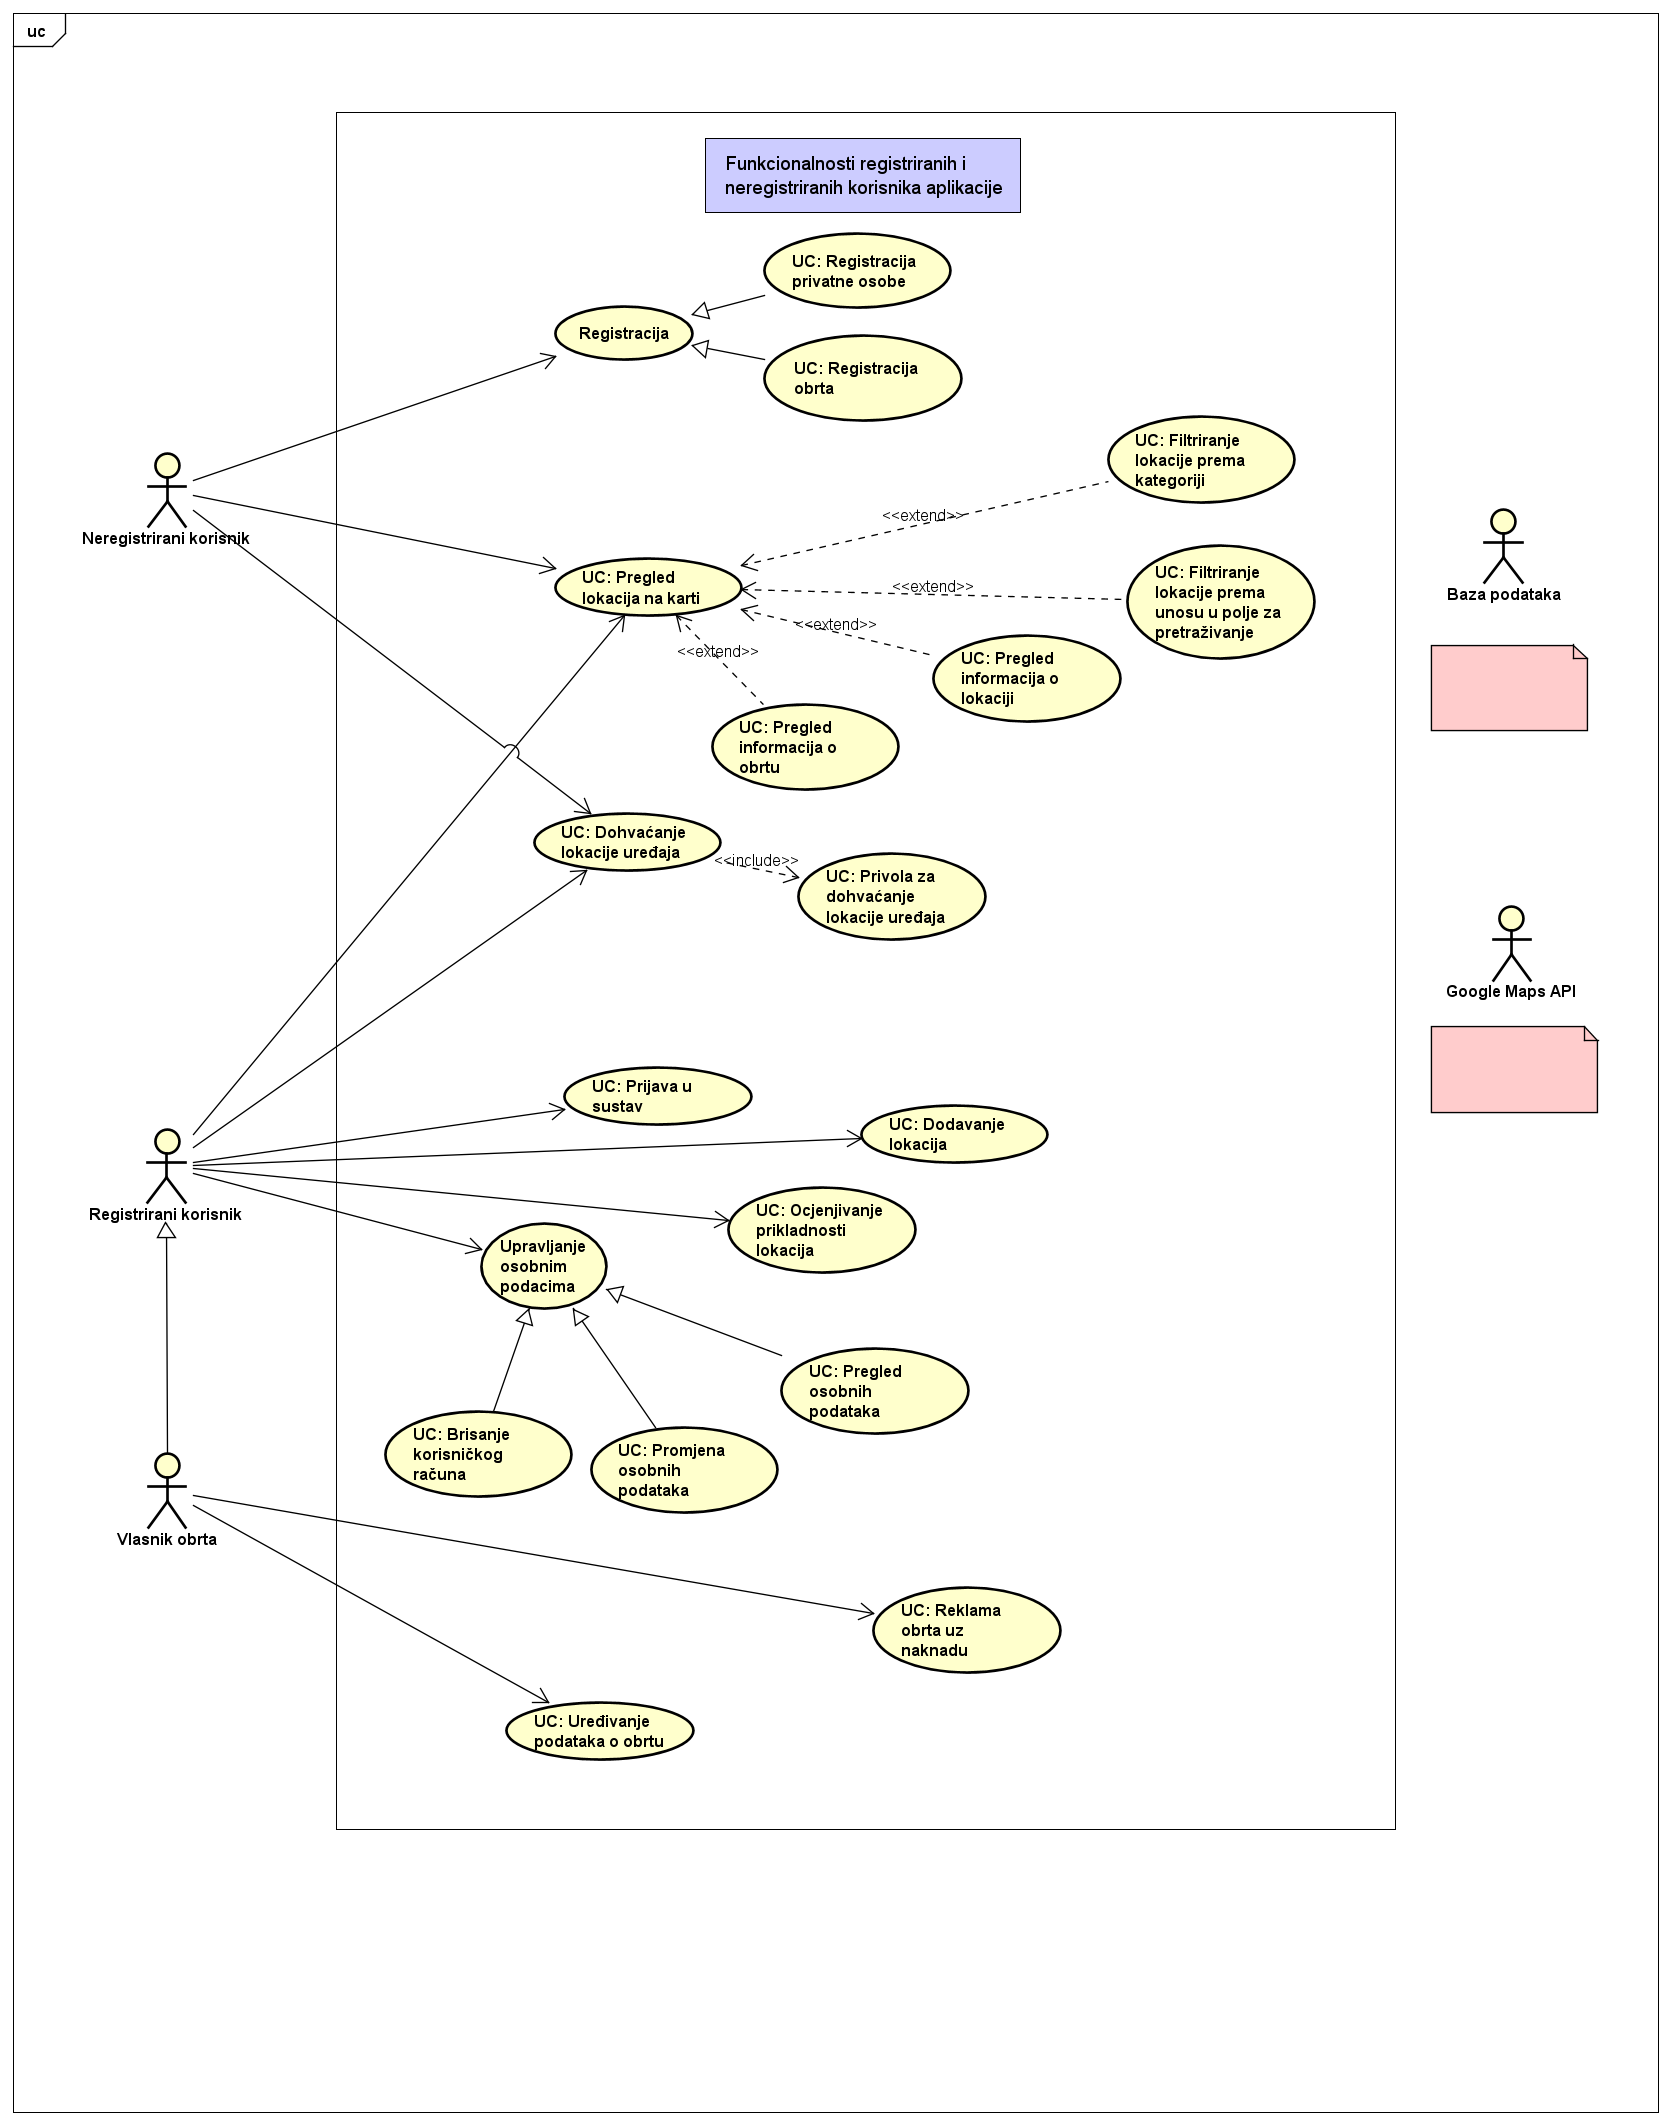
\includegraphics[scale=1.2]{slike/DijagramObrazacaUporabe1.png}
						\centering
						\caption{Dijagram obrazaca uporabe}
						\label{fig:promjene}
					\end{figure}
				\eject		
				
			\subsection{Sekvencijski dijagrami}
				
				\textbf{\textit{dio 1. revizije}}\\
				
				\textit{Nacrtati sekvencijske dijagrame koji modeliraju najvažnije dijelove sustava (max. 4 dijagrama). Ukoliko postoji nedoumica oko odabira, razjasniti s asistentom. Uz svaki dijagram napisati detaljni opis dijagrama.}
				\eject
	
		\section{Ostali zahtjevi}
		
			\textbf{\textit{dio 1. revizije}}\\
		 
			 \textit{Nefunkcionalni zahtjevi i zahtjevi domene primjene dopunjuju funkcionalne zahtjeve. Oni opisuju \textbf{kako se sustav treba ponašati} i koja \textbf{ograničenja} treba poštivati (performanse, korisničko iskustvo, pouzdanost, standardi kvalitete, sigurnost...). Primjeri takvih zahtjeva u Vašem projektu mogu biti: podržani jezici korisničkog sučelja, vrijeme odziva, najveći mogući podržani broj korisnika, podržane web/mobilne platforme, razina zaštite (protokoli komunikacije, kriptiranje...)... Svaki takav zahtjev potrebno je navesti u jednoj ili dvije rečenice.}
			 
			 
			 
	
	\chapter{Arhitektura i dizajn sustava}
            \noindent Arhitektura se može podijeliti na četiri podsustava:
            \begin{packed_item}
	
        	\item  Web poslužitelj
        	\item  Web aplikacija
        	\item  Baza podataka
            \item  Servis za autentifikaciju
            \end{packed_item}
            \\
            
\textit{Web preglednik} je program koji korisniku omogućuje pregled web-stranica i multimedijalnih sadržaja vezanih uz njih. Svaki internetski preglednik je prevoditelj. Dakle, stranica je pisana u kodu koji preglednik nakon toga interpretira kao nešto svakome razumljivo. Korisnik putem web preglednika šalje zahtjev web poslužitelju.
\begin{figure}[H]
	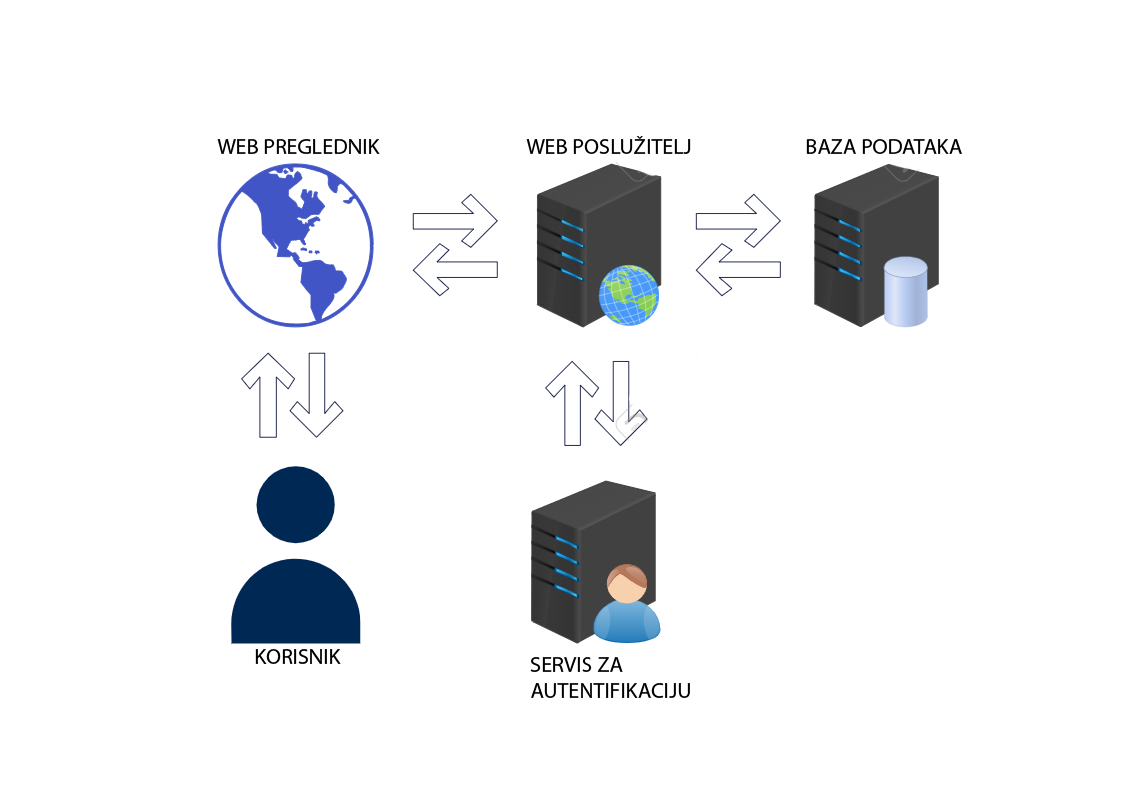
\includegraphics[scale=0.4]{slike/ArhitekturaSustava.png} 
	\centering
	\caption{Prikaz arhitekture}
	\label{fig:promjene}
\end{figure}

\newline
\\
\textit{Web poslužitelj} osnova je rada web aplikacije. Njegova primarna zadaća je komunikacija klijent s aplikacijom. Komunikacija se odvija preko HTTP (engl. \textit{Hyper Text Transfer Protocol}) protokola, što je protokol u prijenosu informacija na webu. Poslužitelj je onaj koji pokreće web aplikaciju te joj prosljeđuje zahtjeve.
\newline
\\
Korisnik korisi \textit{web aplikaciju} za obrađivanje željenih zahtjeva. Web aplikacija obrađuje zahtjev te ovisno o zahtjevu, pristupa bazi podataka i/ili servisu za autentifikaciju nakon čega preko poslužitelja vraća korisniku odgovor u obliku HTML dokumenta vidljivog u web pregledniku.
\newline
\\
Programski jezik kojeg smo odabrali za izradu naše web aplikacije je JavaScript za koji koristimo React biblioteku (engl. \textit{library}) te Next.js radni okvir (engl. \textit{framework}. Za autentifikaciju koristimo Google-ov modul za autentifikaciju iz njihovog servisa Firebase. Odabrano razvojno okruženje je Microsoft Visual Studio Code. Iako ne potpuno, arhitektura sustava temeljit će se na MVC (Model-View-Controller) konceptu. MVC koncept nije potpuno podržan od strane Next.js-a jer je to radni okvir koji omogućava posluživanje React aplikacija sa servera, a u samom React-u MVC koncept nije potpuno podržan. No, radi lakše izrade i organizacije projekta, odlučili smo na što bliži način implementirati MVC koncept.
\newline
\\
Karakteristika MVC koncepta je nezavisan razvoj pojedinih dijelova aplikaicje što za posljedicu ima jednostasvnije ispitivanje kao i jednostsavno razvijanje i dodavanje novih svojstava u sustav.
\newline
\\
MVC koncept sastoji se od:

\begin{packed_item}
	
        	\item  \textbf{Model} - Središnja komponenta sustava. Predstavlja dinamičke strukture podataka, neovisne o korisničkom sučelju. Izravno upravlja podacima, logikom i pravilima aplikacije. Također prima ulazne podatke od Controllera
        	\item \textbf{View} - Bilo kakav prikaz podataka, poput grafa. Mogući su različiti prikazi iste informacije poput grafičkog ili tabličnog prikaza podataka.
        	\item  \textbf{Controller} - Prima ulaze i prilagođava ih za prosljeđivanje Modelu i Viewu. Upravlja korisničkim zahtjevima i zemeljem njih izvodi daljnju interakciju s ostalim elementima sustava.
            \end{packed_item}


	
		

		

				
		\section{Baza podataka}

  Za potrebe našeg sustava koristit ćemo Firestore, Google-ovu NoSQL cloud bazu podataka iz njihovog servisa Firebase koja svojom strukturom omogućava lake izmijene koje će pratiti skaliranje aplikacije. Gradivna jedinka baze je kolekcija (engl. \textit{collection}) definirana svojim imenom i skupom dokumenata (engl. \textit{documents}). Zadaća baze podataka je brza i jednostavna pohrana, izmjena i dohvat podataka za daljnju obradu. Baza podataka ove aplikacije sastoji se od sljedećih kolekcija:
  \begin{packed_item}
	
        	\item  users
        	\item  companies
        	\item  locations
            \end{packed_item}
		
			\subsection{Opis tablica}
			
				
				
				\textbf{Users}\hspace{1cm}  Ova tablica sadrži sve relevantne informacije za korisnike aplikacije. Sadrži atribute: UserId, Username, email i verified(boolean atribut koji nam govori je li korisnik verificirao svoj račun). Tablica je u vezi \textit{One-to-One} s tablicom Companies i u vezi \textit{One-to-Many} je s tablicom Locations. 

                
                \begin{longtblr}[
					label=none,
					entry=none
					]{
						width = \textwidth,
						colspec={|X[6,l]|X[6, l]|X[20, l]|}, 
						rowhead = 1,
					} %definicija širine tablice, širine stupaca, poravnanje i broja redaka naslova tablice
					\hline {\textbf{Users}}	 \\ \hline[3pt]
					\SetCell{LightGreen}UserId & VARCHAR	&  	Hashirani string jedinstven za svakog korisnika  	\\ \hline
					Username	& VARCHAR & Nadimak pod kojim će se korisnik predstavljati u aplikaciji  	\\ \hline 
					email & VARCHAR &  E-mail adresa korisnika \\ \hline 
					CompanyOwner & BOOLEAN	&  True ako je korisnik vlasnik obrta, inače False		\\ \hline  
				\end{longtblr}
                \textbf{Locations} \hspace{1cm} Ova tablica sadrži informacije o lokacijama dodanih od strane korisnika. Sadrži atribute: Ime lokacije, id korisnika koji je dodao lokaciju, status prikladnosti i koordinate. U vezi  \textit{Many-to-One} je s tablicom Users.
                \begin{longtblr}[
					label=none,
					entry=none
					]{
						width = \textwidth,
						colspec={|X[6,l]|X[6, l]|X[20, l]|}, 
						rowhead = 1,
					} %definicija širine tablice, širine stupaca, poravnanje i broja redaka naslova tablice
					\hline {\textbf{Locations}}	 \\ \hline[3pt]
					\SetCell{LightGreen}Name & VARCHAR	&  Ime lokacije  	\\ \hline
					\SetCell{LightBlue} UserId	& VARCHAR &  Hashirani string niz jedinstven za korisnika koji je dodao lokaciju 	\\ \hline  
					Prikladna & BOOLEAN	&  True ako je prikladna za ljubimce, inače False		\\ \hline 
                    Coordinates & VARCHAR &  Koordinate lokacije \\ \hline 
				\end{longtblr}
                \textbf{Companies} \hspace{1cm} Ova tablica sadrži informacije o dodanim obrtima. Posjeduje atribute: OIB obrta, Id vlasnika obrta, adresu, naziv obrta, kojoj kategoriji pripada i kratki opis obrta.  U vezi  \textit{One-to-One} je s tablicom Users.
                \begin{longtblr}[
					label=none,
					entry=none
					]{
						width = \textwidth,
						colspec={|X[6,l]|X[6, l]|X[20, l]|}, 
						rowhead = 1,
					} %definicija širine tablice, širine stupaca, poravnanje i broja redaka naslova tablice
					\hline {\textbf{Companies}}	 \\ \hline[3pt]
					\SetCell{LightGreen}OIB & VARCHAR	&  Niz od 11 znamenki karakterističan za tu pravnu osobu  	\\ \hline
					\SetCell{LightBlue} OwnerId	& VARCHAR &  Hashirani string niz jedinstven za korisnika koji je ujedino i vlasnik obrta 	\\ \hline  
					Adress & VARCHAR	&  Adresa obrta	\\ \hline 
                    Name & VARCHAR &  Ime obrta \\ \hline 
                    Type & VARCHAR &  Kategorija kojoj obrt pripada \\ \hline 
                    Phone & VARCHAR &  Kontakt broj obrta\\ \hline 
					Description & VARCHAR &  Kratki opis obrta \\ \hline 
				\end{longtblr}

                
				
				
			
			\subsection{Dijagram baze podataka}
				\textit{ U ovom potpoglavlju potrebno je umetnuti dijagram baze podataka. Primarni i strani ključevi moraju biti označeni, a tablice povezane. Bazu podataka je potrebno normalizirati. Podsjetite se kolegija "Baze podataka".}
                %oznaci kljuceve
				Na dijagramu ključevi su "boldani", a strani ključevi podcrtani.
                \begin{figure}[H]
			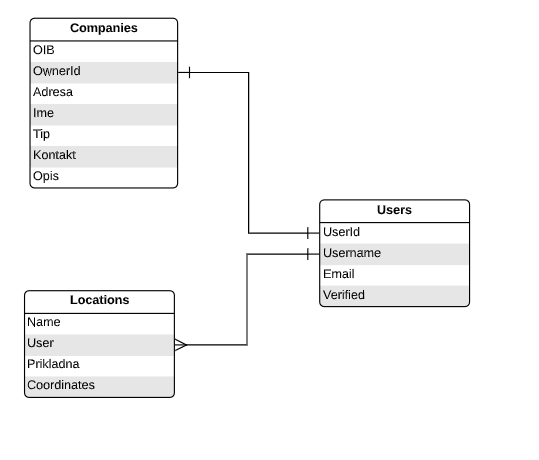
\includegraphics[scale=1.2]{slike/Baza.png}
			\centering
			\caption{Dijagram baze podataka}
			\label{fig:promjene}
		          \end{figure}
			
			\eject
			
		\section{Dijagram razreda}
		
			
			\begin{figure}[H]
			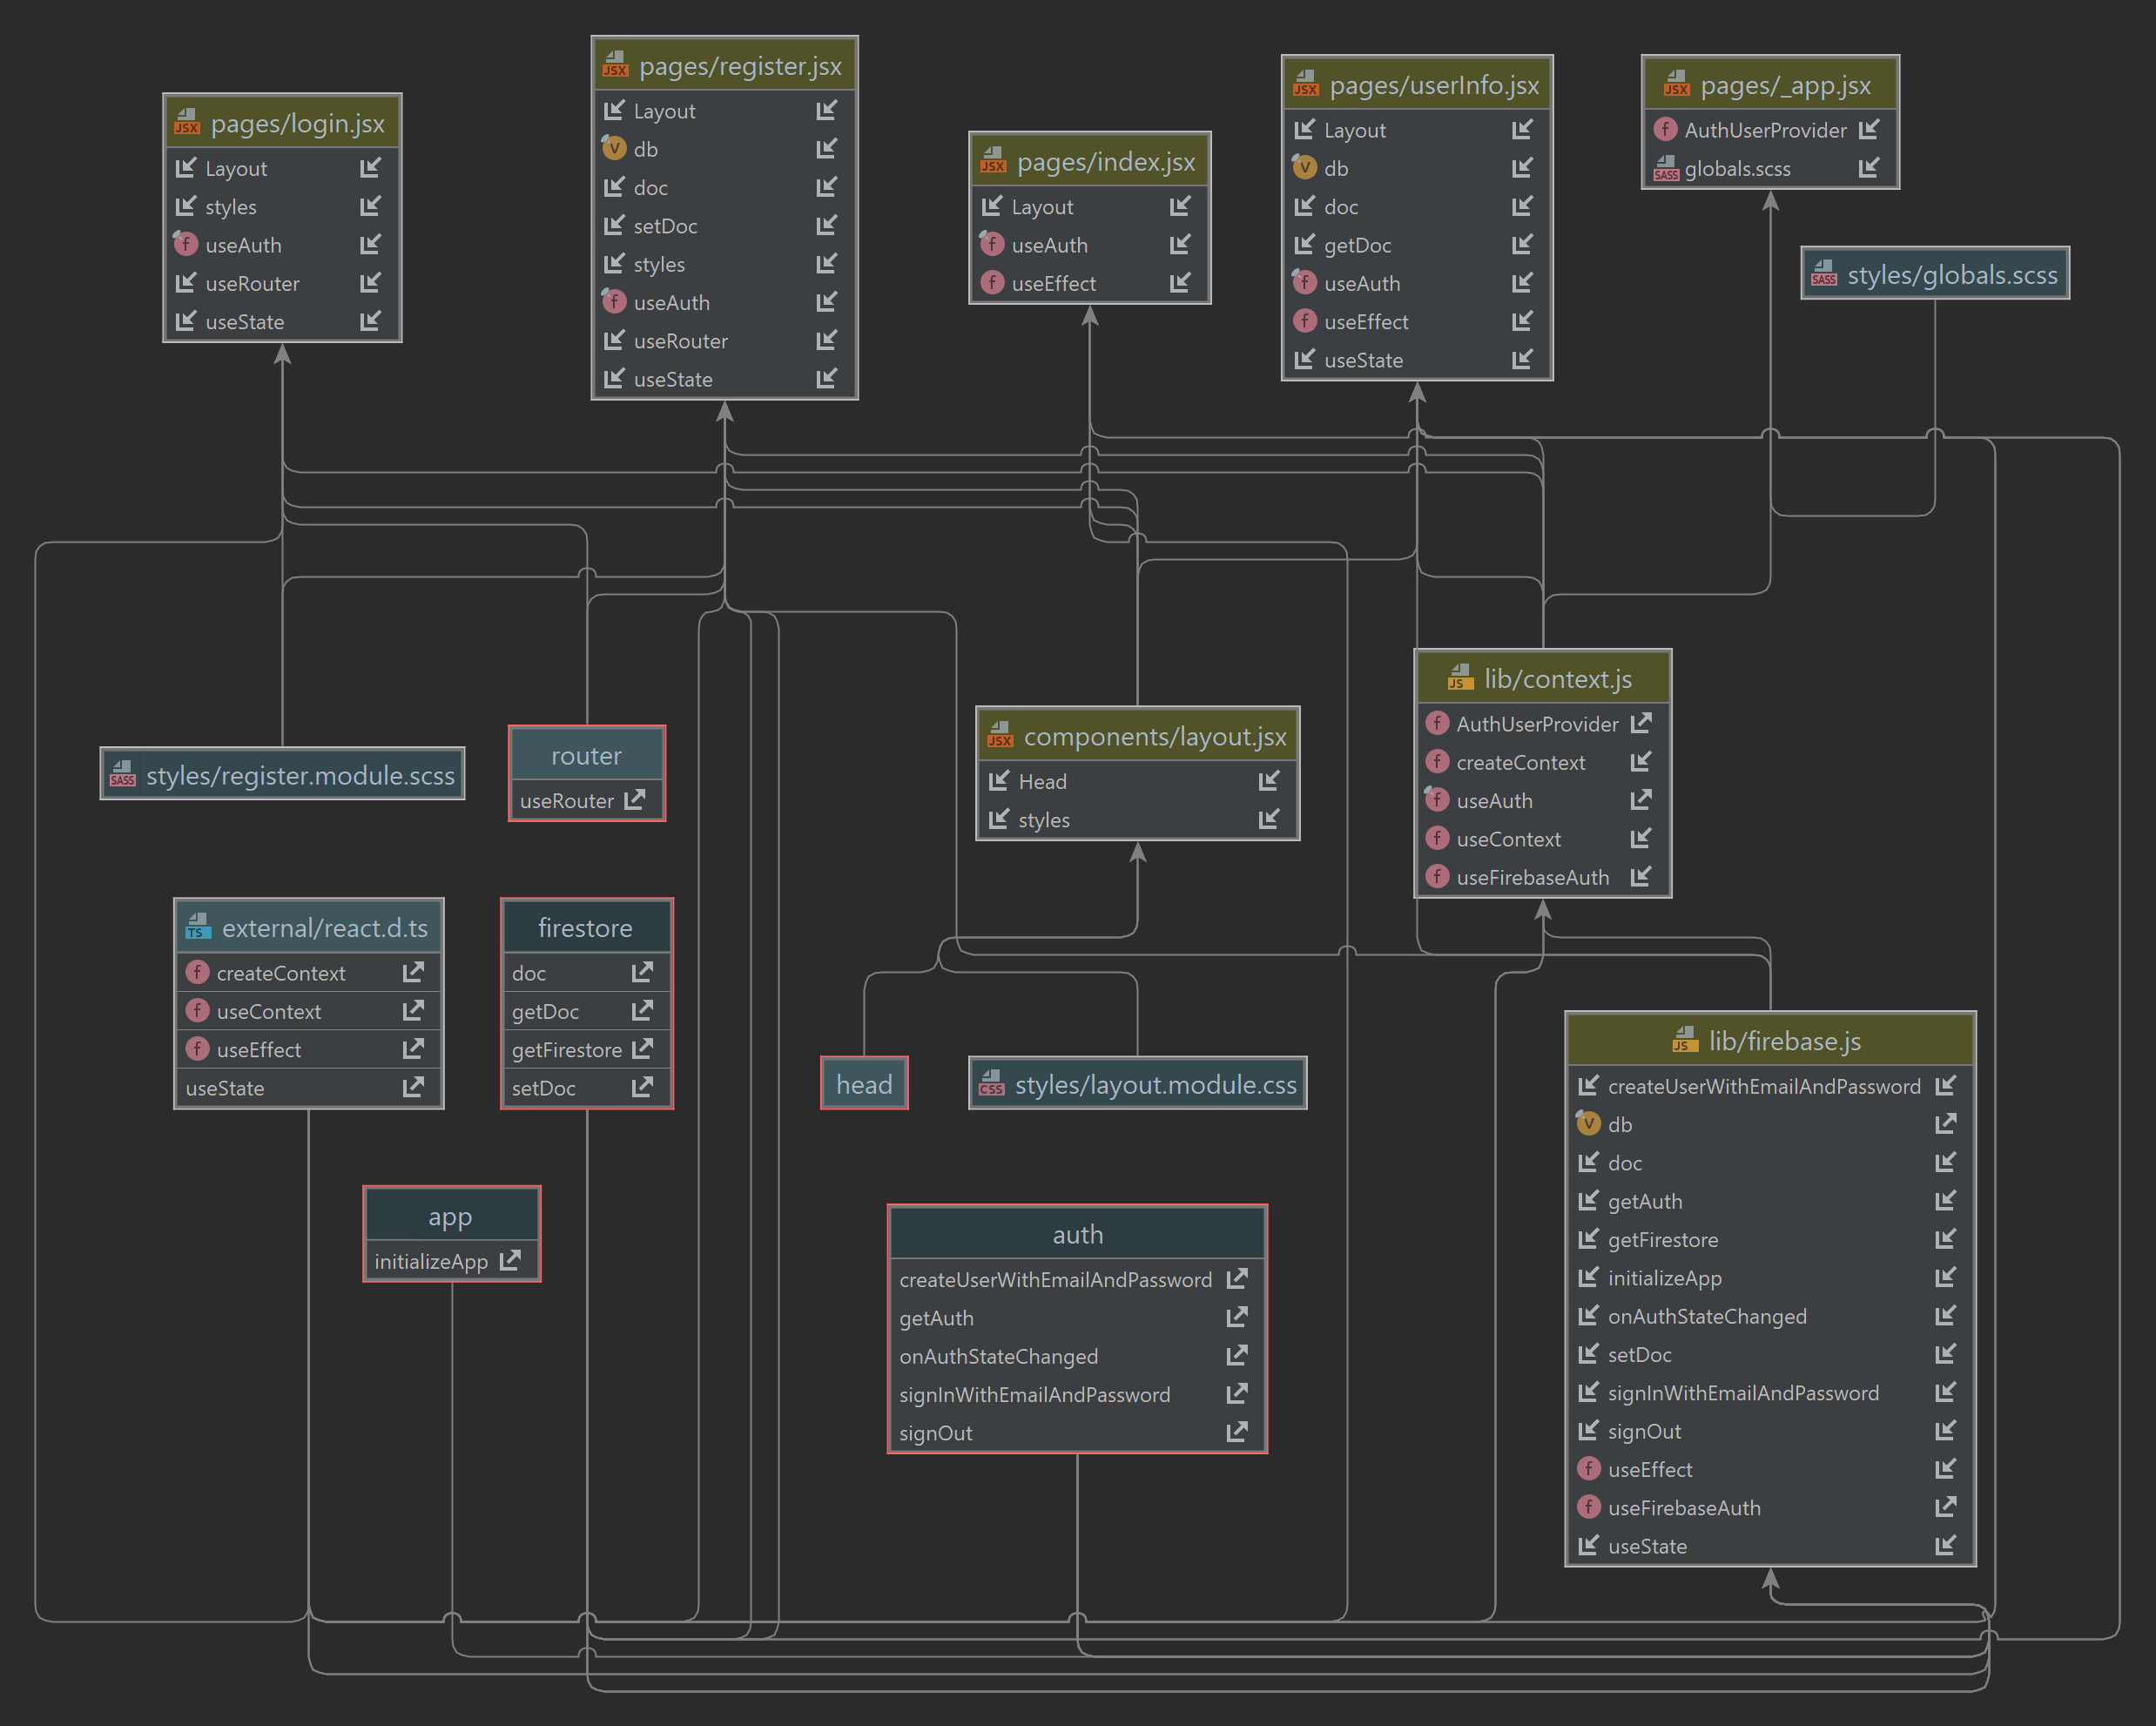
\includegraphics[scale=0.2]{slike/UMLDijagram.png}
			\centering
			\caption{UML Dijagram}
			\label{fig:promjene}
		          \end{figure}
			
			Na slici 4.3 prikazan je dijagram razreda cijelog projekta. Implementirane metode direktno komuniciraju s bazom podataka te vraćaju tražene podatke.
			
			PrivatnaForm.jsx služi za unos informacija o privatnom korisniku, vrši provjeru ispravnosti unosa i ako je sve u redu kreira korisnika u firebaseu
			
			VlasnikForm.jsx služi za unos informacija o obrtu. Sadrži podatke potrebne za neki obrt, provjerava ispravnost unesenih podataka i ako je sve u redu kreira korisnika u firebaseu.
	
	        Firebase.js služi za konfiguraciju baze i komunikaciju s istom. 
	        
	        Context.js stvara kontekst za trenutnog korisnika
	        
	        Hook.js provjerava nalazi li se lozinka u "password blacklisti" i ako da, traži promjenu lozinke.
	        
	        Login.jsx korisniku prikazuje stranicu za ulogiravanje u aplikaciju. Prilikom log-ina gleda se postoji li korisnik u bazi, ako ne javlja se greška. Ako postoji ulogirava se u aplikaciju. Ne dozvoljava se upis dok sva polja nisu ispravno upisana.
	        
	        Register.jsx korisniku prikazuje stranicu za registraciju. U zavisnisti od odabranog prikazuje se ili "PrivatnaForma" ili "VlasnikForma"
	        
	        UseInfo.jsx prikazuje stranicu sa podatcima o ulogiranom korisniku. Prvotno funkcija povlači podatke o korisniku iz baze i ako je korisnik vlasnik firme, povlači i podatke o firmi. Te se isti podatci prikazuju na stranici
	        
	        \begin{figure}[H]
			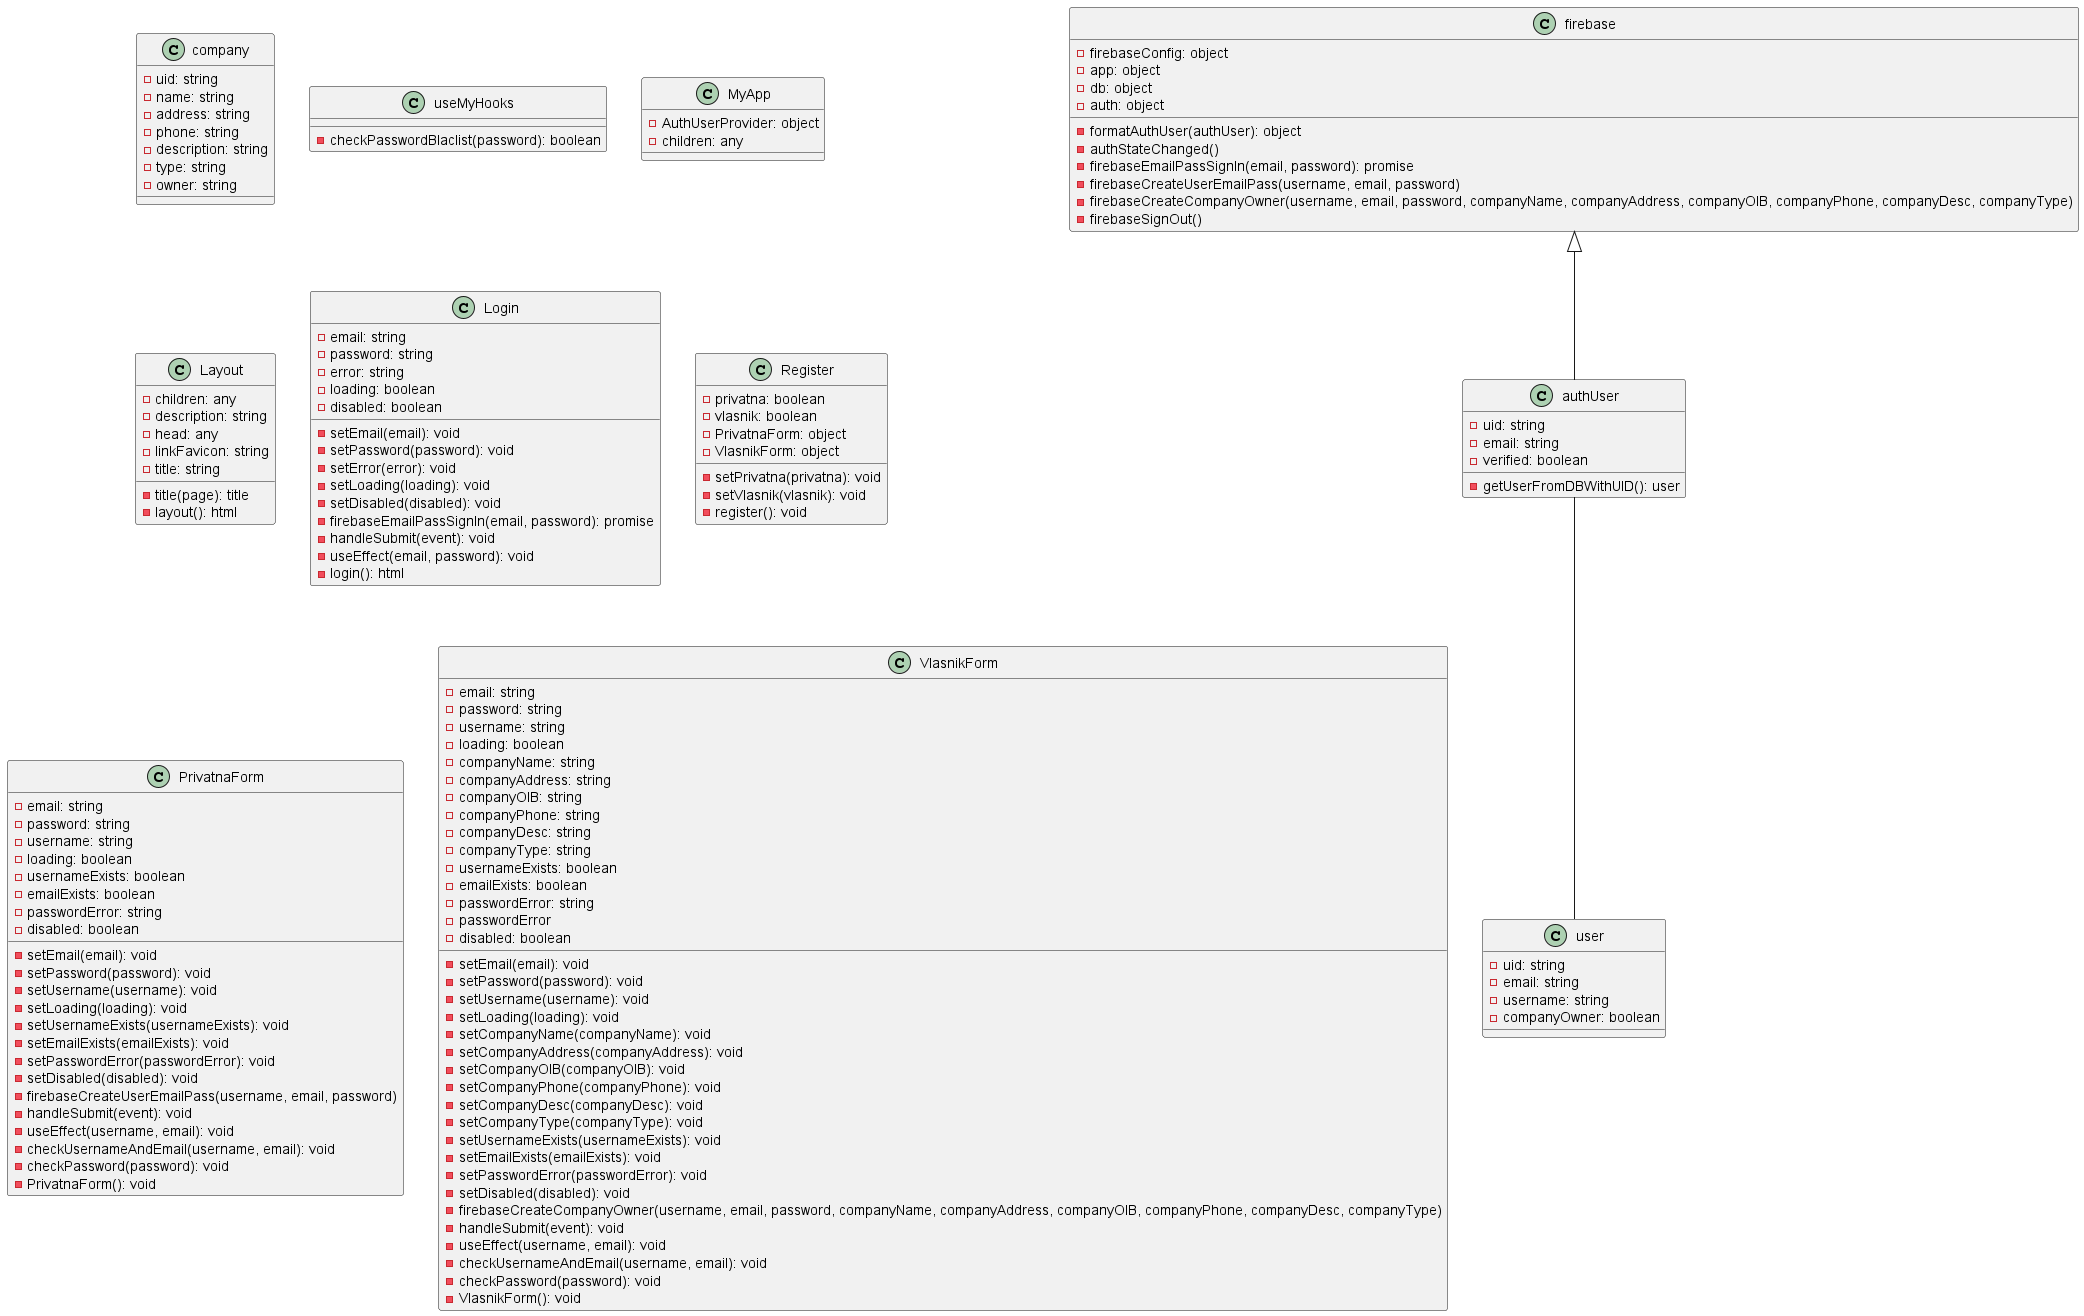
\includegraphics[scale=0.2]{dokumentacija/slike/modeli_iz_baze.png}
			\centering
			\caption{Modeli iz Baze}
			\label{fig:promjene}
		          \end{figure}
			
			%\textbf{\textit{dio 2. revizije}}\\			
			
			%\textit{Prilikom druge predaje projekta dijagram razreda i opisi moraju odgovarati stvarnom stanju implementacije}
			
			
			
			%\eject
		
		%\section{Dijagram stanja}
			
			
			%\textbf{\textit{dio 2. revizije}}\\
			
			%\textit{Potrebno je priložiti dijagram stanja i opisati ga. Dovoljan je jedan dijagram stanja koji prikazuje \textbf{značajan dio funkcionalnosti} sustava. Na primjer, stanja korisničkog sučelja i tijek korištenja neke ključne funkcionalnosti jesu značajan dio sustava, a registracija i prijava nisu. }
			
			
			%\eject 
		
		%\section{Dijagram aktivnosti}
			
			%\textbf{\textit{dio 2. revizije}}\\
			
			% \textit{Potrebno je priložiti dijagram aktivnosti s pripadajućim opisom. Dijagram aktivnosti treba prikazivati značajan dio sustava.}
			
			%\eject
		%\section{Dijagram komponenti}
		
			%\textbf{\textit{dio 2. revizije}}\\
		
			 %\textit{Potrebno je priložiti dijagram komponenti s pripadajućim opisom. Dijagram komponenti treba prikazivati strukturu cijele aplikacije.}
	%\chapter{Implementacija i korisničko sučelje}
		
		
		\section{Korištene tehnologije i alati}
		
			\textbf{\textit{dio 2. revizije}}
			
			 \textit{Detaljno navesti sve tehnologije i alate koji su primijenjeni pri izradi dokumentacije i aplikacije. Ukratko ih opisati, te navesti njihovo značenje i mjesto primjene. Za svaki navedeni alat i tehnologiju je potrebno \textbf{navesti internet poveznicu} gdje se mogu preuzeti ili više saznati o njima}.
			
			
			\eject 
		
	
		\section{Ispitivanje programskog rješenja}
			
			\textbf{\textit{dio 2. revizije}}\\
			
			 \textit{U ovom poglavlju je potrebno opisati provedbu ispitivanja implementiranih funkcionalnosti na razini komponenti i na razini cijelog sustava s prikazom odabranih ispitnih slučajeva. Studenti trebaju ispitati temeljnu funkcionalnost i rubne uvjete.}
	
			
			\subsection{Ispitivanje komponenti}
			\textit{Potrebno je provesti ispitivanje jedinica (engl. unit testing) nad razredima koji implementiraju temeljne funkcionalnosti. Razraditi \textbf{minimalno 6 ispitnih slučajeva} u kojima će se ispitati redovni slučajevi, rubni uvjeti te izazivanje pogreške (engl. exception throwing). Poželjno je stvoriti i ispitni slučaj koji koristi funkcionalnosti koje nisu implementirane. Potrebno je priložiti izvorni kôd svih ispitnih slučajeva te prikaz rezultata izvođenja ispita u razvojnom okruženju (prolaz/pad ispita). }
			
			
			
			\subsection{Ispitivanje sustava}
			
			 \textit{Potrebno je provesti i opisati ispitivanje sustava koristeći radni okvir Selenium\footnote{\url{https://www.seleniumhq.org/}}. Razraditi \textbf{minimalno 4 ispitna slučaja} u kojima će se ispitati redovni slučajevi, rubni uvjeti te poziv funkcionalnosti koja nije implementirana/izaziva pogrešku kako bi se vidjelo na koji način sustav reagira kada nešto nije u potpunosti ostvareno. Ispitni slučaj se treba sastojati od ulaza (npr. korisničko ime i lozinka), očekivanog izlaza ili rezultata, koraka ispitivanja i dobivenog izlaza ili rezultata.\\ }
			 
			 \textit{Izradu ispitnih slučajeva pomoću radnog okvira Selenium moguće je provesti pomoću jednog od sljedeća dva alata:}
			 \begin{itemize}
			 	\item \textit{dodatak za preglednik \textbf{Selenium IDE} - snimanje korisnikovih akcija radi automatskog ponavljanja ispita	}
			 	\item \textit{\textbf{Selenium WebDriver} - podrška za pisanje ispita u jezicima Java, C\#, PHP koristeći posebno programsko sučelje.}
			 \end{itemize}
		 	\textit{Detalji o korištenju alata Selenium bit će prikazani na posebnom predavanju tijekom semestra.}
			
			\eject 
		
		
		\section{Dijagram razmještaja}
			
			\textbf{\textit{dio 2. revizije}}
			
			 \textit{Potrebno je umetnuti \textbf{specifikacijski} dijagram razmještaja i opisati ga. Moguće je umjesto specifikacijskog dijagrama razmještaja umetnuti dijagram razmještaja instanci, pod uvjetom da taj dijagram bolje opisuje neki važniji dio sustava.}
			
			\eject 
		
		\section{Upute za puštanje u pogon}
		
			\textbf{\textit{dio 2. revizije}}\\
		
			 \textit{U ovom poglavlju potrebno je dati upute za puštanje u pogon (engl. deployment) ostvarene aplikacije. Na primjer, za web aplikacije, opisati postupak kojim se od izvornog kôda dolazi do potpuno postavljene baze podataka i poslužitelja koji odgovara na upite korisnika. Za mobilnu aplikaciju, postupak kojim se aplikacija izgradi, te postavi na neku od trgovina. Za stolnu (engl. desktop) aplikaciju, postupak kojim se aplikacija instalira na računalo. Ukoliko mobilne i stolne aplikacije komuniciraju s poslužiteljem i/ili bazom podataka, opisati i postupak njihovog postavljanja. Pri izradi uputa preporučuje se \textbf{naglasiti korake instalacije uporabom natuknica} te koristiti što je više moguće \textbf{slike ekrana} (engl. screenshots) kako bi upute bile jasne i jednostavne za slijediti.}
			
			
			 \textit{Dovršenu aplikaciju potrebno je pokrenuti na javno dostupnom poslužitelju. Studentima se preporuča korištenje neke od sljedećih besplatnih usluga: \href{https://aws.amazon.com/}{Amazon AWS}, \href{https://azure.microsoft.com/en-us/}{Microsoft Azure} ili \href{https://www.heroku.com/}{Heroku}. Mobilne aplikacije trebaju biti objavljene na F-Droid, Google Play ili Amazon App trgovini.}
			
			
			\eject 
	%\chapter{Zaključak i budući rad}
		%komentar
		\textbf{\textit{dio 2. revizije}}\\
		
		 %$\textit{U ovom poglavlju potrebno je napisati osvrt na vrijeme izrade projektnog zadatka, koji su tehnički izazovi prepoznati, jesu li riješeni ili kako bi mogli biti riješeni, koja su znanja stečena pri izradi projekta, koja bi znanja bila posebno potrebna za brže i kvalitetnije ostvarenje projekta i koje bi bile perspektive za nastavak rada u projektnoj grupi.}
		
		% \textit{Potrebno je točno popisati funkcionalnosti koje nisu implementirane u ostvarenoj aplikaciji.}

        Zadatak naše grupe bio je razvoj web aplikacije za prikaz, lociranje i dodavanje lokacija pogodnih za pse. Nakon 17 tjedana rada u timu i razvoja, ostvarili smo zadani cilj. Sama provedba projekta bila je kroz dvije faze.

        Prva faza projekta uključivala je okupljanje tima za razvoj aplikacije, dodjelu projektnog zadatka i rad na dokumentiranju zahtjeva. Kvalitetan rad na prvom dijelu uvelike nam olakšava daljnji rad. 
        
        Druga faza projekta bila je puno intenzivnija po pitanju samostalnog rada članova. Osim realizacije rješenja, u drugoj fazi je bilo potrebno dokumentirati ostale UML dijagrame i izraditi popratnu dokumentaciju kako budući korisnici mogli lakše korisititi ili vršiti preinake na sustavu. Dobro izrađen kostur uštedio nam je puno vremena prilikom izrade aplikacije.
        
        Komunikacija među članovima tima bila je putem Discorda čime smo postigli informiranost i uključenost svih članova grupe. Moguće proširenje postojeće inačice sustava je izrada mobilne aplikacije čime bi cilj projektnog zadatka bio ostvaren u većoj mjeri no s web aplikacijom.
        Sudjelovanje na ovakvom projektu bilo je vrijedno iskustvo svim članovima tima jer smo kroz intenzivnih nekoliko tjedana rada iskusili zajednički rad na istom projektu, te naučili korisitit nove tehnologije. Također, osjetili smo važnost dobre vremenske organiziranosti i koordiniranosti između članova tima. Zadovoljni smo postignutim rezultatom bez obzira na prostor za usavrđavanje izrađene aplikacije.
		
		\eject 
	\chapter*{Popis literature}
		\addcontentsline{toc}{chapter}{Popis literature}
	 	
 		\textbf{\textit{Kontinuirano osvježavanje}}
	
		\textit{Popisati sve reference i literaturu koja je pomogla pri ostvarivanju projekta.}
		
		
		\begin{enumerate}
			
			
			\item  Programsko inženjerstvo, FER ZEMRIS, \url{http://www.fer.hr/predmet/proinz}

			\item  The Unified Modeling Language, \url{https://www.uml-diagrams.org/}
			
			\item  Astah Community, \url{http://astah.net/editions/uml-new}
		\end{enumerate}
		
		 
	
	
	\begingroup
	\renewcommand*\listfigurename{Indeks slika i dijagrama}
	%\renewcommand*\listtablename{Indeks tablica}
	%\let\clearpage\relax
	\listoffigures
	%\vspace{10mm}
	%\listoftables
	\endgroup
	\addcontentsline{toc}{chapter}{Indeks slika i dijagrama}


	
	\eject 
		
	\chapter*{Dodatak: Prikaz aktivnosti grupe}
		\addcontentsline{toc}{chapter}{Dodatak: Prikaz aktivnosti grupe}
		
		\section*{Dnevnik sastajanja}
		

		\begin{packed_enum}
			\item  sastanak
			
			\item[] \begin{packed_item}
				\item 20.10.2022., 13:45
				\item Prisustvovali: Laura Majer, Petra-Dunja Grujić-Ostojić, Fran Markulin, Karla Udiljak, Branimir Medvedec, Jura Starčević, Luka Radman, Marko Štrk
				\item Teme sastanka: 
				\begin{packed_item}
					\item  sastanak s asistenticom i demonstratoricom
					\item  raščišćavanje osnovnih dilema funkcionalnosti
					\item  analiza zadatka
				\end{packed_item}
			\end{packed_item}
			
			\item  sastanak
			\item[] \begin{packed_item}
				\item Datum: 02.11.2022., 13:00
				\item Prisustvovali: Fran Markulin, Karla Udiljak, Branimir Medvedec, Jura Starčević, Luka Radman, Marko Štrk
				\item Teme sastanka:
				\begin{packed_item}
					\item  podijela dužnosti:
					\begin{packed_item}
						\item  Fran Markulin: voditelj projekta, developer
						\item  Karla Udiljak: designer
						\item  Branimir Medvedec: developer
						\item  Jura Starčević: dokumentacija
						\item  Luka Radman: developer
						\item  Marko Štrk: dokumentacija
					\end{packed_item}
					\item  uvod u tehnologiju i arhitekturu koju bi koristili
					\item  rješavanje pitanja i nedoumica oko tehnologije i arhitekture
					\item  razrada strukture baze podataka
					\item  ostali dogovori
				\end{packed_item}
			\end{packed_item}

			\item  sastanak
			
			\item[] \begin{packed_item}
				\item 05.11.2022., 10:00
				\item Prisustvovali: Fran Markulin, Branimir Medvedec, Luka Radman
				\item Teme sastanka: 
				\begin{packed_item}
					\item  rad na razvoju aplikacije
				\end{packed_item}
			\end{packed_item}

			\item  sastanak
			
			\item[] \begin{packed_item}
				\item 07.11.2022., 18:00
				\item Prisustvovali: Fran Markulin, Branimir Medvedec
				\item Teme sastanka: 
				\begin{packed_item}
					\item  rad na razvoju aplikacije
				\end{packed_item}
			\end{packed_item}

			\item  sastanak
			
			\item[] \begin{packed_item}
				\item 13.11.2022., 15:00
				\item Prisustvovali: Fran Markulin, Karla Udiljak, Branimir Medvedec, Jura Starčević, Luka Radman, Marko Štrk
				\item Teme sastanka: 
				\begin{packed_item}
					\item  dokumentacija - što još treba i kako dokumentirati
					\item svaki član prezentirao svoj dio posla kako bi svi bili upoznati sa svime na projektu
					\item dogovoreni idući koraci
					\item podijela poslova
					\item zadani rokovi
				\end{packed_item}
			\end{packed_item}

			\item  sastanak
			
			\item[] \begin{packed_item}
				\item 15.11.2022, 7:30
				\item Prisustvovali: Fran Markulin, Branimir Medvedec, Luka Radman
				\item Teme sastanka: 
				\begin{packed_item}
					\item  rad na razvoju aplikacije
					\item priprema za prvu predaju
				\end{packed_item}
			\end{packed_item}

			\item  sastanak
			
			\item[] \begin{packed_item}
				\item 16.11.2022., 10:30
				\item Prisustvovali: Fran Markulin, Branimir Medvedec
				\item Teme sastanka: 
				\begin{packed_item}
					\item  komentiranje programskog koda
					\item rad na dokumentaciji
					\item priprema za izradu dijagrama razreda
				\end{packed_item}
			\end{packed_item}

			\item  sastanak
			
			\item[] \begin{packed_item}
				\item 17.11.2022., 13:45
				\item Prisustvovali: Laura Majer, Fran Markulin, Karla Udiljak, Branimir Medvedec, Jura Starčević, Luka Radman, Marko Štrk
				\item Teme sastanka: 
				\begin{packed_item}
					\item   demonstracija generičkih funkcionalnosti
					\item rješavanje nedoumica
				\end{packed_item}
			\end{packed_item}
\item  sastanak
    \item[] \begin{packed_item}
				\item 17.12.2022., 15:00
				\item Prisustvovali: Fran Markulin,  Branimir Medvedec, Luka Radman
				\item Teme sastanka: 
				\begin{packed_item}
					\item   Programiranje
				\end{packed_item}
			\end{packed_item}
\item  sastanak
   \item[] \begin{packed_item}
				\item 18.11.2022., 15:00
				\item Prisustvovali: Fran Markulin,  Branimir Medvedec
				\item Teme sastanka: 
				\begin{packed_item}
					\item  Programiranje
				\end{packed_item}
			\end{packed_item}
			
			%
			
		\end{packed_enum}
		
		\eject
		\section*{Tablica aktivnosti}
		
			%\textbf{\textit{Kontinuirano osvježavanje}}\\
			
			% \textit{Napomena: Doprinose u aktivnostima treba navesti u satima po članovima grupe po aktivnosti.}

			\begin{longtblr}[
					label=none,
				]{
					vlines,hlines,
					width = \textwidth,
					colspec={X[6, l]X[1, c]X[1, c]X[1, c]X[1, c]X[1, c]X[1, c]}, 
					vline{1} = {1}{text=\clap{}},
					hline{1} = {1}{text=\clap{}},
					rowhead = 1,
				} 
				\multicolumn{1}{c|}{} & \multicolumn{1}{c|}{\rotatebox{90}{\textbf{Fran Markulin}}} & \multicolumn{1}{c|}{\rotatebox{90}{\textbf{Branimir Medvedec}}} &	\multicolumn{1}{c|}{\rotatebox{90}{\textbf{Luka Radman}}} & \multicolumn{1}{c|}{\rotatebox{90}{\textbf{Karla Udiljak }}} &	\multicolumn{1}{c|}{\rotatebox{90}{\textbf{ Jura Starčević}}} & \multicolumn{1}{c|}{\rotatebox{90}{\textbf{Marko Štrk }}}  \\  
				Upravljanje projektom 		&48  &  &  &  &  &   \\ 
				Opis projektnog zadatka 	&  &  &  &  &6  &   \\ 
				
				Funkcionalni zahtjevi       & 1 &  &  & 1 &1.5  &    \\ 
				Opis pojedinih obrazaca 	&  &  &  &  &  &  7  \\ 
				Dijagram obrazaca 			&  &  &  & 4 &  &    \\ 
				Sekvencijski dijagrami 		&  &  &  &6  &  &    \\ 
				Opis ostalih zahtjeva 		&  &  &  &  &  & 2.5  \\ 

				Arhitektura i dizajn sustava	 &3  &  &  &  & 4.5  &    \\ 
				Baza podataka				&3  &  &  &  & 3 &    \\ 
				Dijagram razreda 			&6  &  & 2 &  &  &  2  \\ 
				Dijagram stanja				&  &  &  & 2.5 &  &   \\ 
				Dijagram aktivnosti 		&  &  &  & 2.5 &  &    \\ 
				Dijagram komponenti			&  &  &  & 2.5 &  &    \\ 
				Korištene tehnologije i alati 		&  &  &  &  &2  &    \\ 
				Ispitivanje programskog rješenja 	4&  &  &  &  &1  &   \\ 
				Dijagram razmještaja			&  &  &  & 1  &  &    \\ 
				Upute za puštanje u pogon 		&  &  &  &  &  &  1 \\  
				Zaključak i budući rad 		&  &  &  &  &  &1    \\  
				Popis literature 			& 0.5 &  &  &  &1  &   \\  
                Izrada login stranice			& 2 & 8 &  &  &  &   \\
                Izrada register stranice			& 2 & 6 & 5 &  &  &   \\
                Izrada komponente VlasnikForm			& 3 & 6 & 6 &  &  &   \\
                Izrada komponente PrivatnaForm			& 3 & 4 & 3 &  &  &   \\
                Izrada user info stranice			& 2 & 4 & 8 &  &  &   \\
                Izrada komunikacije s bazom podataka			& 6 &  &  &  &  &   \\
                Izrada konteksta			& 2 &  &  &  &  &   \\
                Izrada komponente layout			& 1 &  &  &  &  &   \\
                Izrada posebnih funkcija (hook.js)  & 1 &  &  &  &  &   \\
                Izrada baze podataka  & 4 &  &1  &  &  &   \\
                Vođenje git repotizorija & 9 &  &  &  &  &   \\
                Dizajn &  &  &  & 32 &  &   \\
                Dnevnik sastajanja & 1 &  &  &  &1  &   \\
                Moderiranje Latex dokumenta & 1 &  &  &  &35  & 1\\
                Izrada Index stranice   & 24 &  &  &  &  &   \\
                Izrada tests stranice  & 8 &  &  &  &  &   \\
                Izrada PaymentForm  &  & 17 &  &  &  &   \\
                Izrada Index-Home  &  & 7 &  &  &  &   \\
                
	\end{longtblr}

	
					
					
		\eject
		\section*{Dijagrami pregleda promjena}
		\begin{figure}[H]
			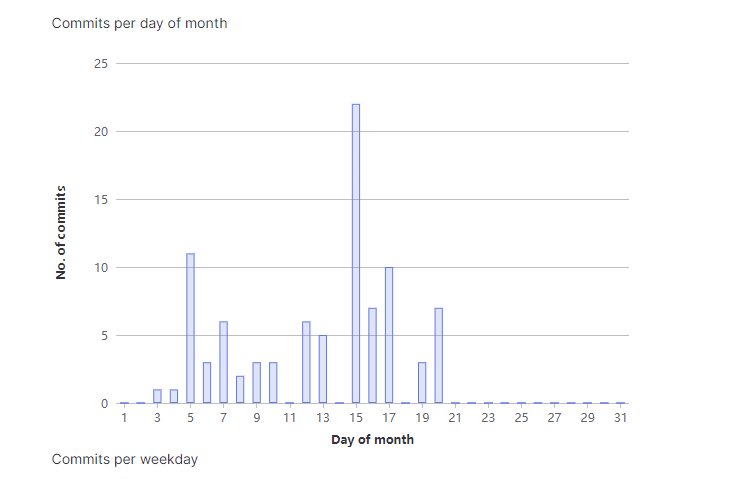
\includegraphics[scale=0.7]{slike/commits.png}
			\centering
			\caption{Prikaz aktivnosti u projektu}
			\label{fig:promjene}
		          \end{figure}
		%\textbf{\textit{dio 2. revizije}}\\
		
		%\textit{Prenijeti dijagram pregleda promjena nad datotekama projekta. Potrebno je na kraju projekta generirane grafove s gitlaba prenijeti u ovo poglavlje dokumentacije. Dijagrami za vlastiti projekt se mogu preuzeti s gitlab.com stranice, u izborniku Repository, pritiskom na stavku Contributors.}
		
	


\end{document} %naredbe i tekst nakon ove naredbe ne ulaze u izgrađen dokument 


